\documentclass[letter, 11pt]{article}
%% ================================
%% Packages =======================
\usepackage[utf8]{inputenc}      %%
\usepackage[T1]{fontenc}         %%
\usepackage{lmodern}             %%
\usepackage[spanish]{babel}      %%
\decimalpoint                    %%
\usepackage{fullpage}            %%
\usepackage{fancyhdr}            %%
\usepackage{graphicx}            %%
\usepackage{amsmath}             %%
\usepackage{color}               %%
\usepackage{mdframed}            %%
\usepackage[colorlinks]{hyperref}%%
%% ================================
%% ================================

%% ================================
%% Page size/borders config =======
\setlength{\oddsidemargin}{0in}  %%
\setlength{\evensidemargin}{0in} %%
\setlength{\marginparwidth}{0in} %%
\setlength{\marginparsep}{0in}   %%
\setlength{\voffset}{-0.5in}     %%
\setlength{\hoffset}{0in}        %%
\setlength{\topmargin}{0in}      %%
\setlength{\headheight}{54pt}    %%
\setlength{\headsep}{1em}        %%
\setlength{\textheight}{8.5in}   %%
\setlength{\footskip}{0.5in}     %%
%% ================================
%% ================================

%% =============================================================
%% Headers setup, environments, colors, etc.
%%
%% Header ------------------------------------------------------
\fancypagestyle{firstpage}
{
  \fancyhf{}
  \lhead{
\includegraphics[height=4.5em]{LogoDFI.jpg}}
  \rhead{FI3104-1 \semestre\\
         Métodos Numéricos para la Ciencia e Ingeniería\\
         Prof.: \profesor}
  \fancyfoot[C]{\thepage}
}

\pagestyle{plain}
\fancyhf{}
\fancyfoot[C]{\thepage}
%% -------------------------------------------------------------
%% Environments -------------------------------------------------
\newmdenv[
  linecolor=gray,
  fontcolor=gray,
  linewidth=0.2em,
  topline=false,
  bottomline=false,
  rightline=false,
  skipabove=\topsep
  skipbelow=\topsep,
]{ayuda}
%% -------------------------------------------------------------
%% Colors ------------------------------------------------------
\definecolor{gray}{rgb}{0.5, 0.5, 0.5}
%% -------------------------------------------------------------
%% Aliases ------------------------------------------------------
\newcommand{\scipy}{\texttt{scipy}}
%% -------------------------------------------------------------
%% =============================================================
%% =============================================================================
%% CONFIGURACION DEL DOCUMENTO =================================================
%% Llenar con la información pertinente al curso y la tarea
%%
\newcommand{\tareanro}{09}
\newcommand{\fechaentrega}{30/11/2017 23:59 hrs}
\newcommand{\semestre}{2018B}
\newcommand{\profesor}{Valentino González}
%% =============================================================================
%% =============================================================================


\begin{document}
\thispagestyle{firstpage}

\begin{center}
  {\uppercase{\LARGE \bf Tarea \tareanro}}\\
  Fecha de entrega: \fechaentrega
\end{center}


%% =============================================================================
%% ENUNCIADO ===================================================================
\noindent{\large \bf Problema 1}

Estime la posición del centro de masa de un sólido descrito por la
intersección de un toro y un cilindro dados por las siguientes ecuaciones:

\begin{align}
  {\rm Toro} : z^2 + \left( \sqrt{x^2 + y^2} - 3 \right)^2 &\leq 1\\
  {\rm Cilindro} : (x - 2)^2 + z^2 &\leq 1
\end{align}

La densidad del sólido varía según la siguiente ecuación:

$$ \rho(x, y, z) = 0.5 \times (x^2 + y^2 + z^2) $$

Resuelva el problema usando alguno de los métodos de integración de Monte
Carlo, para ello debe definirse un volúmen lo más pequeño posible que englobe
al sólido sobre el cual quiere integrar.

Debido a la naturaleza aleatoria del algoritmo, la determinación que haga tiene
una incertidumbre asociada. Para estimar la incertidumbre, repita el
experimento un {\it número grande de veces} y reporte el valor medio y su
desviación estándar. ¿Cómo se comporta el error en función del número de puntos
utilizados para la estimación del volumen?

\begin{ayuda}
  \small
  \noindent {\bf Ayuda.}

  Le puede ser útil mirar la sección ``Simple Monte Carlo Integration'' del
  libro ``Numerical Reicpes in C'', disponible gratis en el siguiente
  \href{http://apps.nrbook.com/c/index.html}{link}.

\end{ayuda}

\vspace{1em}
\noindent{\large \bf Problema 2}

La función de Schechter se usa comúnmente en Astronomía para parametrizar la
Función de Luminosidad (FL) de las galaxias, esto es, la distribución en número
por unidad de volumen por unidad de luminosidad de las galaxias. Su forma es la
siguiente:


$$ \Phi(L) dL = \phi^* \left( \frac{L}{L^*}\right)^\alpha
                \exp\left(- \frac{L}{L^*}\right) dL$$

\noindent donde $\Phi(L)dL$ es la densidad de galaxias con luminosidad entre
$L$ y $L+dL$. $\phi^*$, $L^*$, y $\alpha$ son los parámetros de la función. Por
ejemplo, la Figura \ref{fig:LF}, a) muestra la FL para un set de parámetros
estimados experimentalmente para un grupo de galaxias.

\begin{figure}
  \centering
  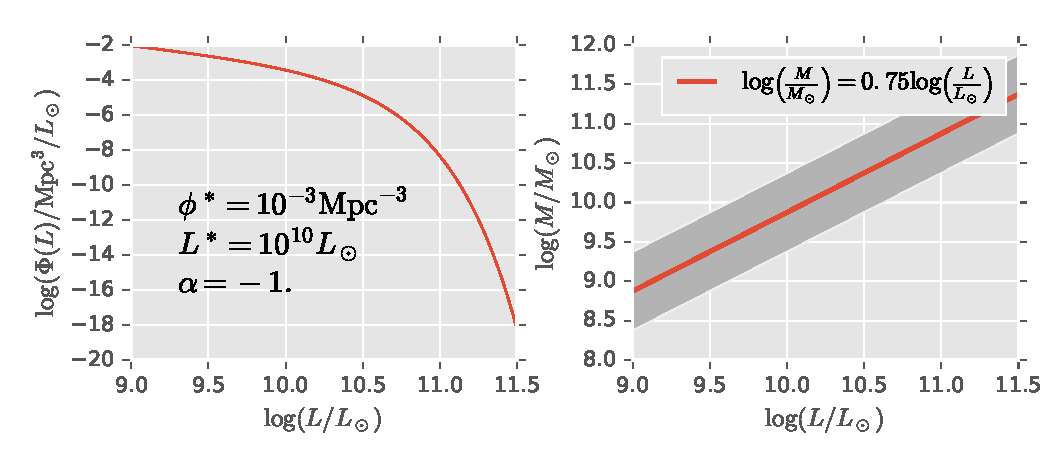
\includegraphics[width=0.8\textwidth]{lf.pdf}
  \caption{a) Función de Luminosidad. b) Relación entre luminosidad y masa.}
  \label{fig:LF}
\end{figure}

En el panel b) de la figura, hay una estimación de la masa de una galaxia como
función de su luminosidad. Como se aprecia, hay una relación lineal, entre
$log(L)$ y $log(M)$ con una incertidumbre asociada. De este modo, dada la
luminosidad de una galaxia, se puede modelar su masa como una variable
aleatoria que se distribuye como una distribución normal $\mathcal{N}(log(M),
0.5^2)$, donde $log(M)$ es una función de $log(L)$ (la función está dada en la
figura).

Su objetivo, es obtener una estimación de la densidad de galaxias con masa
$M=10^{11} M_\odot$ (que corresponde más o menos a la masa en estrellas de la
Vía Láctea).

Estos son los pasos que deberá seguir para resolver el problema:

\begin{enumerate}

\item Considere la FL con los parámetros dados en la Figura \ref{fig:LF}, a).
  Utilícela como si fuera una función densidad de probabilidad. Cree una
  muestra aleatoria de luminosidades sacada de esa distribución. Como consejo,
  parta con un tamaño pequeño para la muestra y vaya agrandándolo. Compruebe
  que la muestra que creó se distribuye como la función de Schechter ploteando
  un histograma de la muestra y la función de Schechter encima. Piense bien en
  cómo se debe normalizar el histograma y la función de Schechter y en qué
  rango de valores de la luminosidad debe crear la muestra.

\item A cada una de las luminosidades de la muestra aleatoria creada
  anteriormente, asígnele ahora su masa correspondiente. Recuerde que su masa
  es una variable aleatoria, asi que tiene que tomar un valor para la masa
  sacado de la distribución correspondiente.

\item Ahora construya el equivalente a la FL pero reemplazando luminosidad por
  masa (eso se llama la función de masa, FM). Lo que acaba de hacer es obtener
  la densidad de galaxias por intervalo de masa.

\item Evalúe esa función para $M=10^{11} M_\odot$. (Puede requerir alguna
  interpolación y otro mecanismo.)

\item Dada la naturaleza aleatoria del procedimiento, la estimación que Ud.
  obtuvo tiene un error asociado. Repita los pasos $1-4$ un número grande de
  veces para estimar el valor medio de la densidad y su desviación estándar.

\end{enumerate}

\begin{ayuda}
  \small
  \noindent {\bf Nota sobre las unidades.}

  Las luminosidades están expresadas en $L_\odot$, esto es, la luminosidad del
  Sol. De igual forma, las masas están expresadas en $M_\odot$, la masa del
  Sol. Los volúmenes están medidos en ${\rm Mpc^3}$, mega parsecs cúbicos.
\end{ayuda}

%%%%%%%%%%%%%%%%%%%%%%%%%%%%%%%%%%%%%%%%%%%%%%%%%%%%%%%%%%%%%%%%%%%%%%%%%%%%%%%
%%%%%%%%%%%%%%%%%%%%%%%%%%%%%%%%%%%%%%%%%%%%%%%%%%%%%%%%%%%%%%%%%%%%%%%%%%%%%%%

\pagebreak
\noindent\textbf{Instrucciones Importantes.}
\begin{itemize}

\item Evaluaremos su uso correcto de \texttt{python}. Si define una función
  relativametne larga o con muchos parámetros, recuerde escribir el
  \emph{docstring} que describa los parámetros que recibe la función, el
  output, y el detalle de qué es lo que hace la función. Recuerde que
  generalmente es mejor usar varias funciones cortas (que hagan una sola cosa
  bien) que una muy larga (que lo haga todo).  Utilice nombres explicativos
  tanto para las funciones como para las variables de su código. El mejor
  nombre es aquel que permite entender qué hace la función sin tener que leer
  su implementación ni su \emph{docstring}.

\item Su código debe aprobar la guía sintáctica de estilo
  (\href{https://www.python.org/dev/peps/pep-0008/}{\texttt{PEP8}}). En
  \href{http://pep8online.com}{esta página} puede chequear si su código aprueba
  \texttt{PEP8}.

\item Utilice \texttt{git} durante el desarrollo de la tarea para mantener un
  historial de los cambios realizados. La siguiente
  \href{https://education.github.com/git-cheat-sheet-education.pdf}{cheat
    sheet} le puede ser útil. {\bf Revisaremos el uso apropiado de la
  herramienta y asignaremos una fracción del puntaje a este ítem.} Realice
  cambios pequeños y guarde su progreso (a través de \emph{commits})
  regularmente. No guarde código que no corre o compila (si lo hace por algún
  motivo deje un mensaje claro que lo indique). Escriba mensajes claros que
  permitan hacerse una idea de lo que se agregó y/o cambió de un
  \texttt{commit} al siguiente.

\item Al hacer el informe usted debe decidir qué es interesante y agregar las
  figuras correspondientes. No olvide anotar los ejes, las unidades e incluir
  una \emph{caption} o título que describa el contenido de cada figura.

\item La tarea se entrega subiendo su trabajo a github. Trabaje en el código y
  en el informe, haga \textit{commits} regulares y cuando haya terminado
  asegúrese de hacer un último \texttt{commit} y luego un \texttt{push} para
  subir todo su trabajo a github. \textbf{REVISE SU REPOSITORIO PARA ASEGURARSE
  QUE SUBIÓ LA TAREA. SI UD. NO PUEDE VER SU INFORME EN GITHUB.COM, TAMPOCO
PODREMOS NOSOTROS.}

\item El informe debe ser entregado en formato \texttt{pdf}, este debe ser
  claro sin información de más ni de menos. \textbf{Esto es muy importante, no
  escriba de más, esto no mejorará su nota sino que al contrario}. La presente
  tarea probablemente no requiere informes de más de 2 páginas más un montón de
  figuras.  Asegúrese de utilizar figuras efectivas y tablas para resumir sus
  resultados. Revise su ortografía.

 \item Repartición de puntaje: 40\% implementación y resolución de los
   problemas (independiente de la calidad de su código); 10\% diseño del
   código: modularidad, uso efectivo de nombres de variables y funciones,
   docstrings, \underline{uso de git}, etc.; 45\% calidad del reporte
   entregado: demuestra comprensión de los problemas y su solución, claridad
   del lenguaje, calidad de las figuras utilizadas; 5\% aprueba a no
   \texttt{PEP8}. Ambas preguntas tienen igual peso en la nota final.


\end{itemize}

%% FIN ENUNCIADO ===============================================================
%% =============================================================================

\end{document}
